\subsection{Arhitektuur}
\subsubsection{Programmi navigeerimine}
Programmil on 2 peamist akent – käivitus ja moodulite aknad. Programm käivitub, kuvades kasutajale akna, kuhu kasutaja peab videofaili sisestama. Pärast faili andmist suunatakse kasutaja moodulite aknale. Moodulite aken sisaldab nuppude võrgustikku kõigi rakenduse saadaolevate funktsioonidega, nagu lõikamine, kärpimine ja filtrid, millele kasutaja pääseb juurde, klõpsates vastavat nuppu. Pildil(\nameref{fig:activityDiagram}) saate protsessi visualiseeriva rakenduse tegevusskeemi.
\begin{figure}[H]
    \centering
    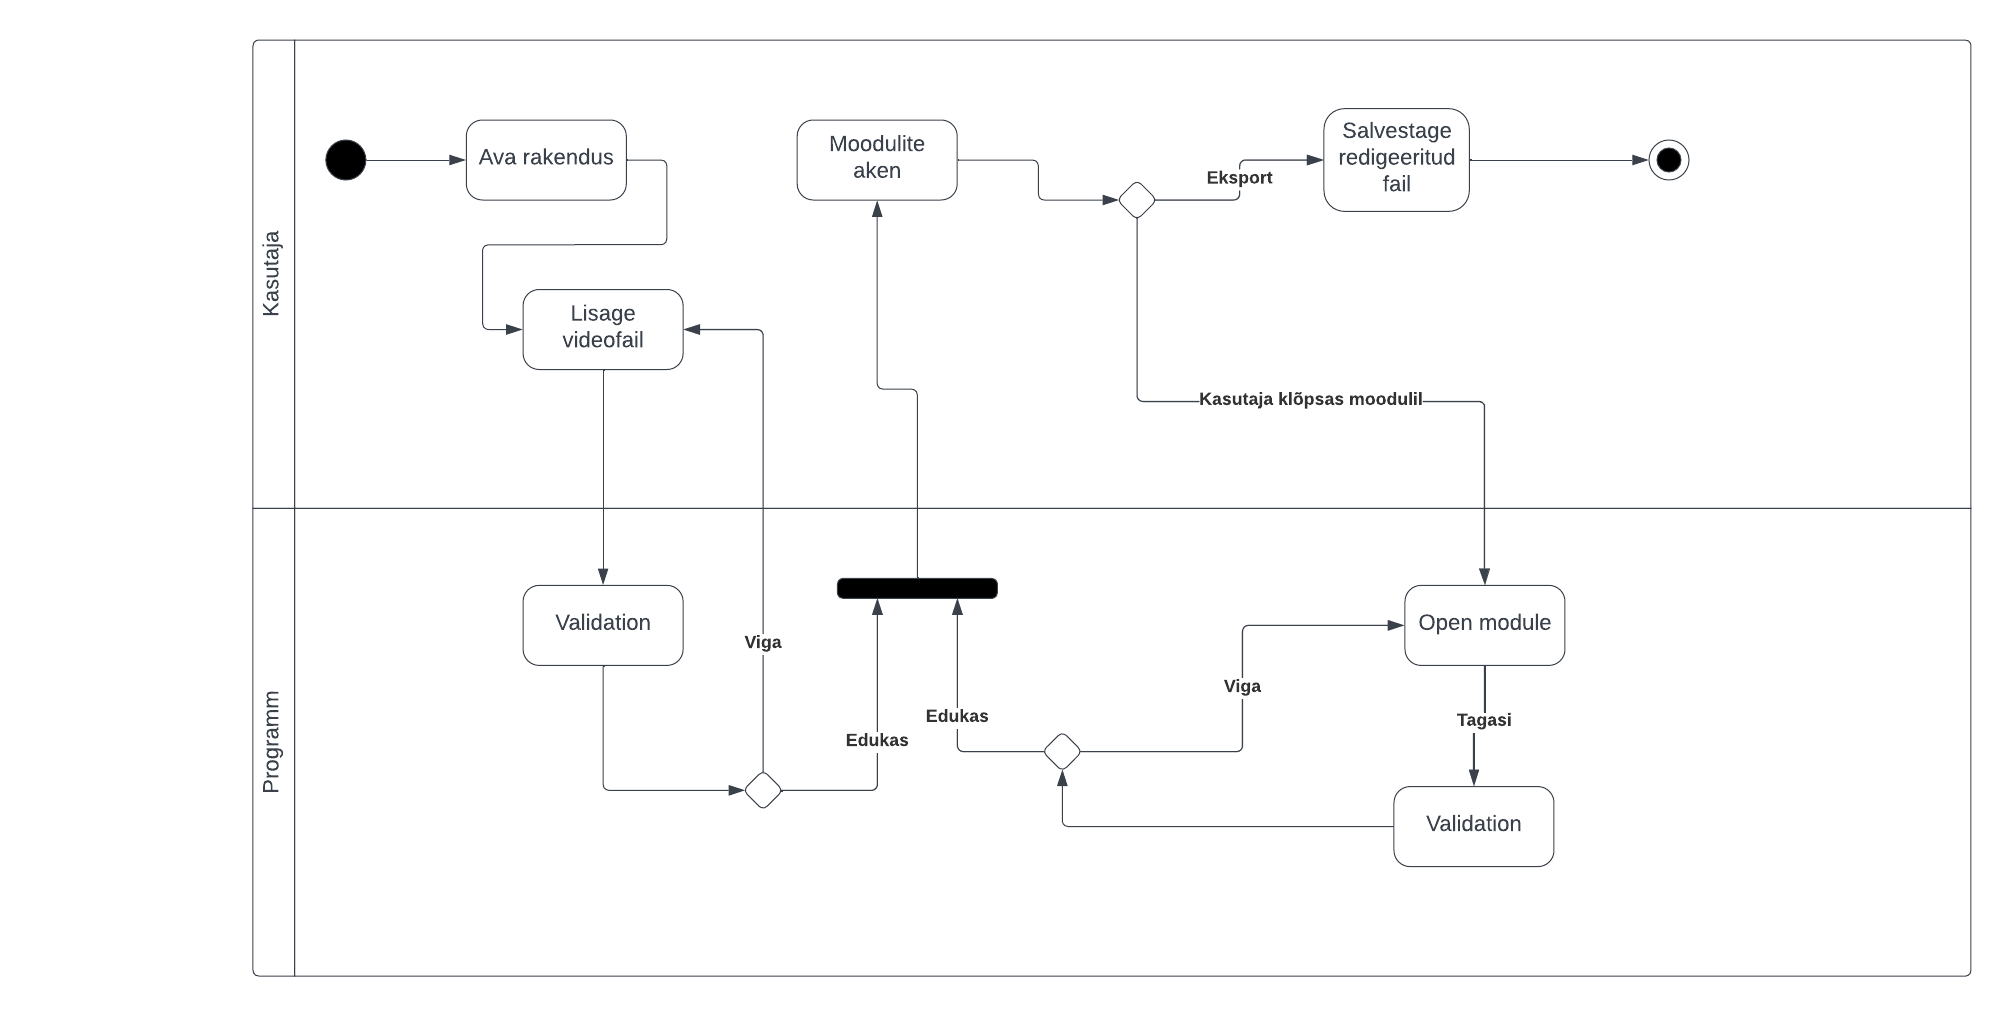
\includegraphics[width=1\textwidth]{Images/Projekti Tegevusskeem.png}
    \caption{Tegevusskeem}
    \label{fig:activityDiagram}
\end{figure}
\subsubsection{Projekti struktuur}
Projekt koosneb järgmistest failikataloogidest: 
\begin{itemize}
\item     pom.xml - sisaldab teavet projekti kohta ja erinevaid üksikasju konfiguratsioonid, mida Maven kasutab projekti loomiseks
    \item src/main - sisaldab kõik projektidega seaotud failid
    \begin{itemize}
        \item java - projekti allika juur, sisaldab kogu projekti Java koodi
        \begin{itemize}
            \item com/project/\projectFolder  - sisaldab Main.java klassi ja kõiki kontrollereid
            \item module-info.java - moodulifail, mis kirjeldab kõiki sõltuvusi, mida projekt selle käitamiseks vajab
        \end{itemize}
        \item         resources - sisaldab projekti ressursse
        \begin{itemize}
        \item locale - sisaldab kõiki projekti tõlkeid
            \item videos - sisaldab projekti arendamisel testimiseks kasutatud videoid
            \item images - sisaldab projektis kasutatud pilte ja ikoone
            \item com/project/\projectFolder - sisaldab kõigi akende fxml-faile
        \end{itemize}
    \end{itemize}
\end{itemize}